\subsection{Frontend}\label{subsec:frontend_design}
The mobile application, and the interface for end users, is designed with ease of use and understandability in mind. This however poses two major design challenges. The frontend of Drive-LaB has two responsibilities in the overall system, namely collection and presentation of location data. Neither of these are however trivial.

The data collection is complicated by requiring user interaction. Without additional equipment, it is not possible to automatically detect the beginning and end of a trip. As such, end users are required to manually control when their smartphone should track their movement. Upon ending a trip, a sequence of actions should take place. A series of locations has been obtained, and should be passed on to the API server. In order to achieve this, data should be converted into classes, readable by the API server. Furthermore, trips are packaged into JSON objects which can be received by the REST service hosted on the API server (See section\ref{sec:api_server}). This sequence of events does not require user interaction, and is fully automatable. Summarizing the process of collecting location data, one can gather three different working states for the application:

\begin{itemize}
\item Idle - Ready to track a new trip
\item Tracking - Continually logging new positions
\item Finishing up - Packaging and sending all logged data
\end{itemize}

These working states are made visible through a central button in the application, as seen in \ref{fig:start_stop_finishing_trip}. The progression of working states happens from left to right. "START TUR" (START TRIP) means the application is ready to track a new trip, and invites the user to do so. "STOP TUR" (STOP TRIP) means the application is currently tracking, and invites the user to end the trip when finished. Finally the user is presented with a message, "AFSLUTTER TUR" (FINISHING TRIP), informing the user that the tracking has stopped, but the application is still working. Upon finishing the process of sending the trip to the API server, the application will once again be ready to start a new trip, displaying "START TUR" for the user.
While the logic behind the button is complex, usage is simple and easy to understand. The user only has to define the beginning and end of a trip; the application takes care of the rest.

\begin{figure}[tb]
\centering
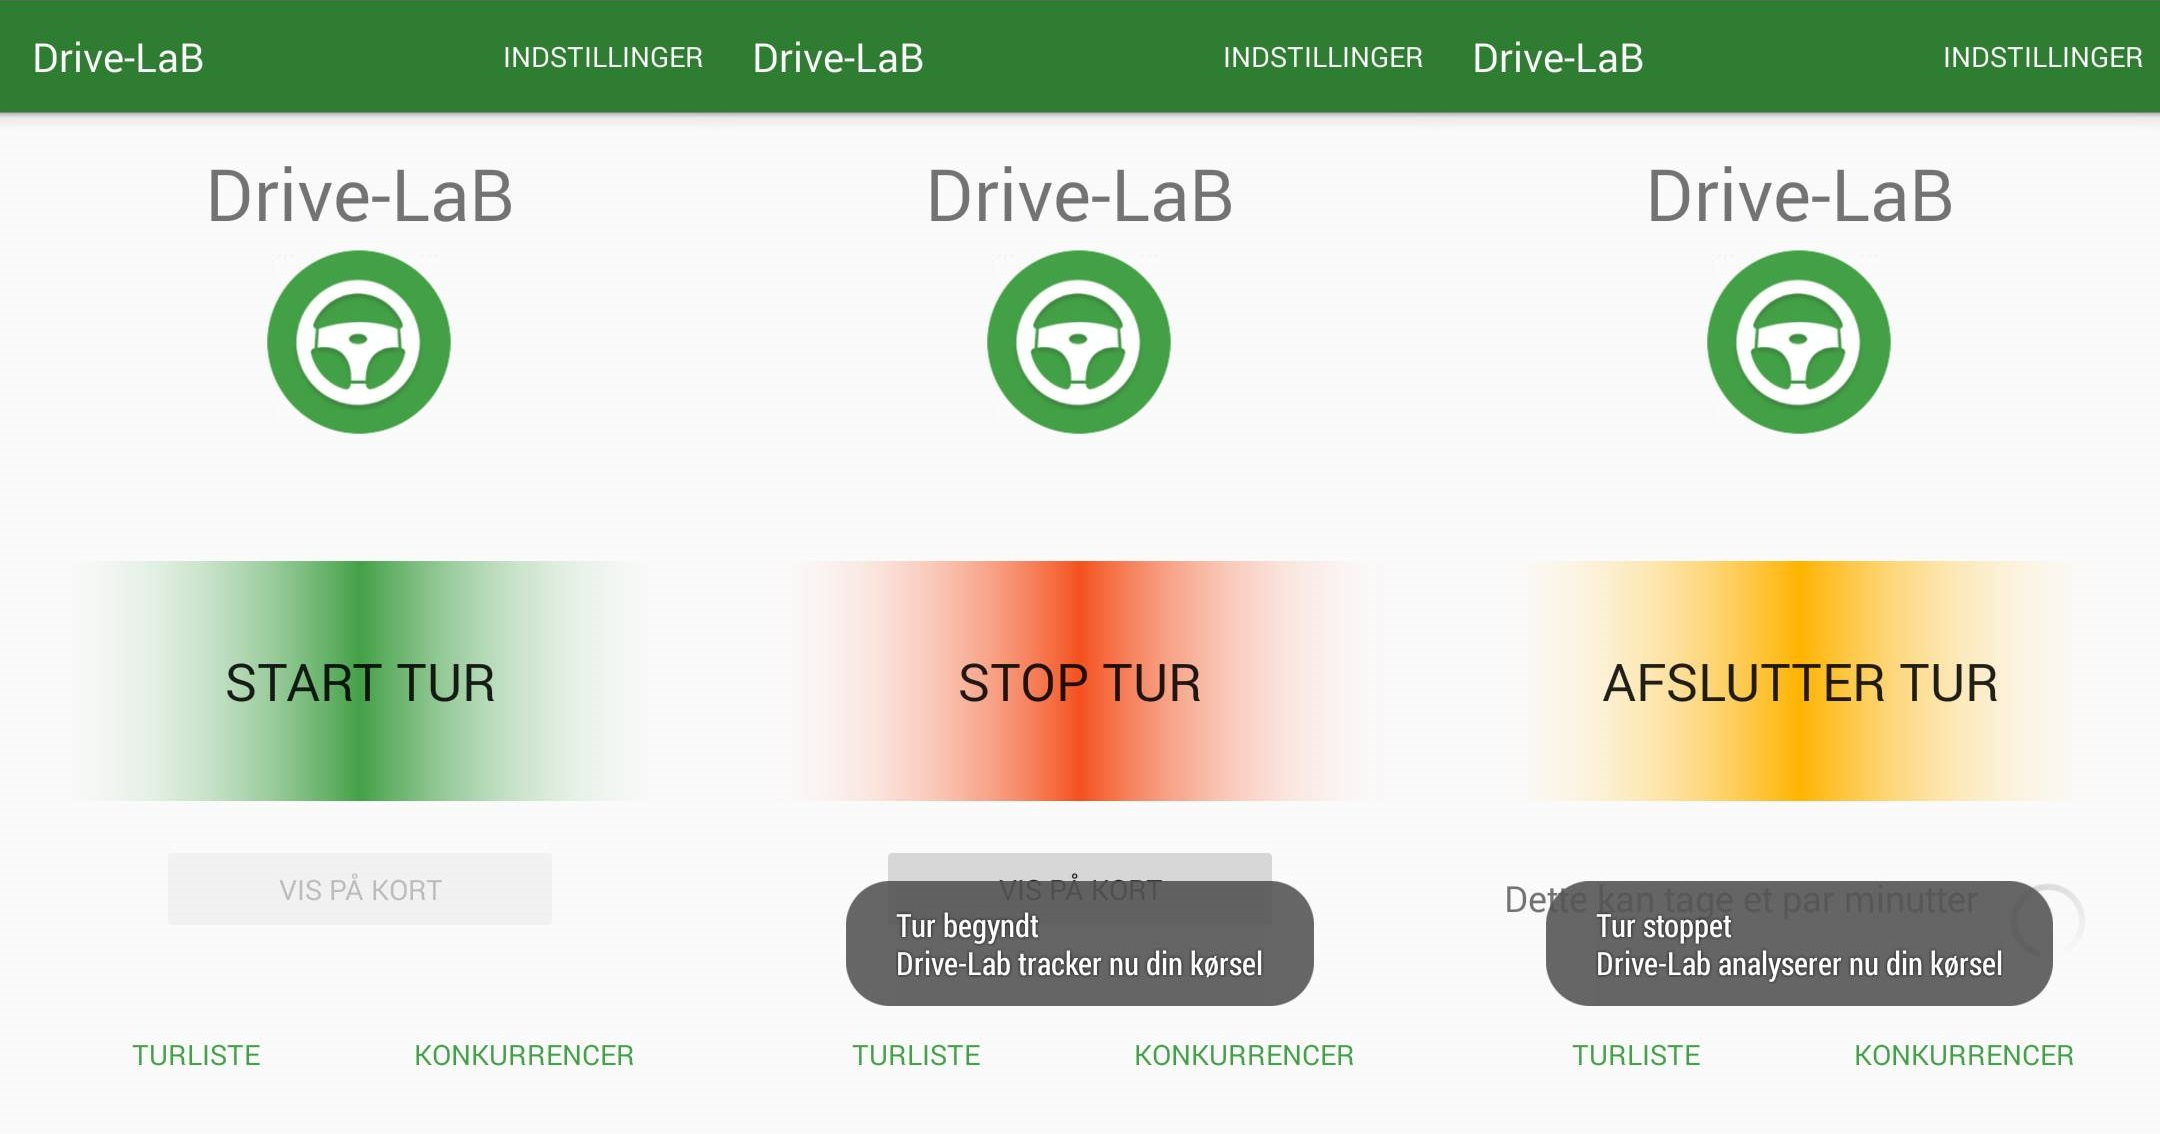
\includegraphics[width=0.465\textwidth]{Pictures/start_stop_finishing_trip}
\caption{Design of the Start/Stop/Finishing button}
\label{fig:start_stop_finishing_trip}
\end{figure}

Data presentation is complicated, both by the extensiveness of the data itself, but also the limited screen size of a smartphone. In other words, the application has to fit a lot of information into a small screen. With the goal of having an easily understandable system, the extensive data is remedied by using descriptive summaries, rather than presenting raw data. The small screen is however still an issue, and for this reason the application offers a multilevel description of trips, each presenting a certain level of data. Each level of description is presented on its own screen, and ranges from a broad description down to specific statistics. For an arbitrary trip, these screens can be seen in \textbf{FIGUR REF}.

Looking at the left screen, users are first presented with a list of all trips showing cursory statistics. These are useful mostly for identifying a trip. In key with keeping Drive-LaB simple to use and understand, the user can also see the trip score summarized as a smiley. The smileys range between green/happy and red/sad. They allow for cursory trip evaluation, without the need to look at more detailed statistics.
The second screen displays a score summary, indicating how metrics affect the base score. The screen clearly visualizes which metrics are problem areas, allowing the user to identify points of possible improval.
The third and fourth screen both shows specifics, and allows the user to see exactly what was registered during a trip. The third screen places the route on a map, showing the user exactly where locations were logged. The fourth screen shows exact metric counts, allowing the user to see why a metric score turned out the way it did.
The different levels of information allow users to only navigate as deep as desired. As such, some users might be satisfied with seeing the resulting smiley, and will not be forced to look at details. For those who want more detailed results however, these are also made available.